%\begin{tcolorbox}[colback=exposed-colour!50,coltext=white,bottom=-35pt]
\chapter{Compartmental models}\label{ch:compartments}
%\end{tcolorbox}
\section{SIR model}
%\paragraph{Introduction}
We begin our study of mathematical epidemiology with the SIR model, a simple deterministic compartmental model that manages to provide some key insights into the spread of infectious disease. Compartmental models split a population into discrete groups called classes or compartments. Making assumptions about how individuals can transfer between these compartments allows us to formulate the systems in terms of differential equations\cite{models-epidemiology}.\\
\\
The SIR model is a special case of the Kermack-McKendrick model that was one of the first mathematical models of epidemics\cite{kermack-mckendrick}. Its simplicity makes it both a good introduction to some concepts and techniques in mathematical epidemiology as well as a flexible template for developing more specialised and nuanced compartmental models.
\subsection{Building the model}
Suppose there is a population of $N$ individuals. Let each individual belong to one of three classes: susceptibles, infective and removed\footnote{The less sinister `recovered' is also used in the literature but is more technically a subset of `removed'.}. They are denoted $S$, $I$ and $R$ respectively. The susceptibles are those who are \textit{at risk} of infection to the disease, the infectives are those who can \textit{currently} spread the disease and the removed can no longer infect others. Individuals who are removed can have already had the infection and recovered with full acquired immunity. They can also have been immunised against the disease, been quarantined or simply died. Whilst to an individual it clearly matters which of these states they are in, they are largely equivalent from the point of view of an applied mathematician.\\
\\
The SIR model supposes that individuals can move from class $S$ to $I$ and from $I$ to $R$. No other movement between classes is possible. Medically, the fact that infective individuals can only move to removed is equivalent to assuming that the disease gives immunity to recovered patients\footnote{A separate class of models called SIS models suppose that no immunisation is bestowed upon recovered patients and they simply move back to the susceptible class. This fundamentally different compartmental structure results in different long term dynamics. Notably SIS models allow the possibility of endemic disease. Endemic disease is a constant presence of disease in a population that does not have outbreaks but also does not die off. As will be seen, this is not possible in the SIR model.}\label{mmd}.\\
\\
Let $S(t),I(t),R(t)$ denote the number of individuals in class $S,I,R$ respectively at time $t$. We now need a host of assumptions to make the problem tractable\cite{models-epidemiology-2}. The first two are to allow us to use partial differential equations:
\begin{enumerate}[noitemsep, label=(\roman*)]
	\item\label{SIR-as-cont} \textit{The number of individuals is a continuous variable}. We assume that we can have fractions of people. This assumption allows us to use differential equations to study the system.
	\item\label{SIR-as-det} \textit{The spread of the epidemic is deterministic}. We assume that the outcome of the epidemic is determined completely by the past history of the system and the rules. This allows us to avoid any element of stochasticity which would suggest the need for more complicated techniques such as stochastic differential equations.
\end{enumerate}
The next assumptions relate to the infection and allow us to simplify the rules of the model:
\begin{enumerate}[resume, noitemsep, label=(\roman*)]
\item\label{SIR-as-pop} \textit{Population size is constant}. So $N=S+I+R$. This can be justified by saying that the time scale of the disease is much shorter than the time scale of demographic change.
\item\label{SIR-as-birth} \textit{There are no births and the only deaths are as a result of the disease}. Note that this is different to \ref{SIR-as-pop} as having a birth for each death would satisfy condition \ref{SIR-as-pop} but lead to different dynamics. Indeed it would amount to introducing a mechanism that allows some members of the removed population to transfer to the susceptible population.\label{mmd}
\item\label{SIR-as-ma} \textit{The law of mass-action applies to contacts between individuals\cite{mass-action}}. The probability of a random contact between two individuals is proportional to the product of the size of each of the groups they belong to. This means that, for example, both an infective and susceptible individual are just as likely to meet an infective individual.
\end{enumerate}
In practice \ref{SIR-as-cont} and \ref{SIR-as-ma} are the most problematic assumptions, particularly for modelling the beginning of the disease. \ref{SIR-as-cont} is acceptable when the population is large and the disease well-established. However at the beginning of a disease outbreak the discrete nature of individuals becomes critical. Similarly \ref{SIR-as-ma} ignores how an outbreak can be avoided by the disease dying out by failing to spread outside of a small infective population. The models in chapter \ref{ch:abms} address these problems by relaxing both of these assumptions as well as \ref{SIR-as-det}. The result is a model that is more effective at describing the outbreak of disease. With this caveat, let's continue.\\
\\
With the set-up described so far and the above assumptions, we can express the rate of change in the size of each class. This results in the system of differential equations:
\begin{eqnarray}
	\dot S=- \beta S I\label{SIR1}\\
	\dot I=\beta S I-\alpha I\label{SIR2}\\
	\dot R=\alpha I\label{SIR3}
\end{eqnarray}
\text{with initial conditions: }$S(0)=S_0\geq0, I(0)=I_0\geq0, R(0)=0$\\
\begin{figure}
	\centering
	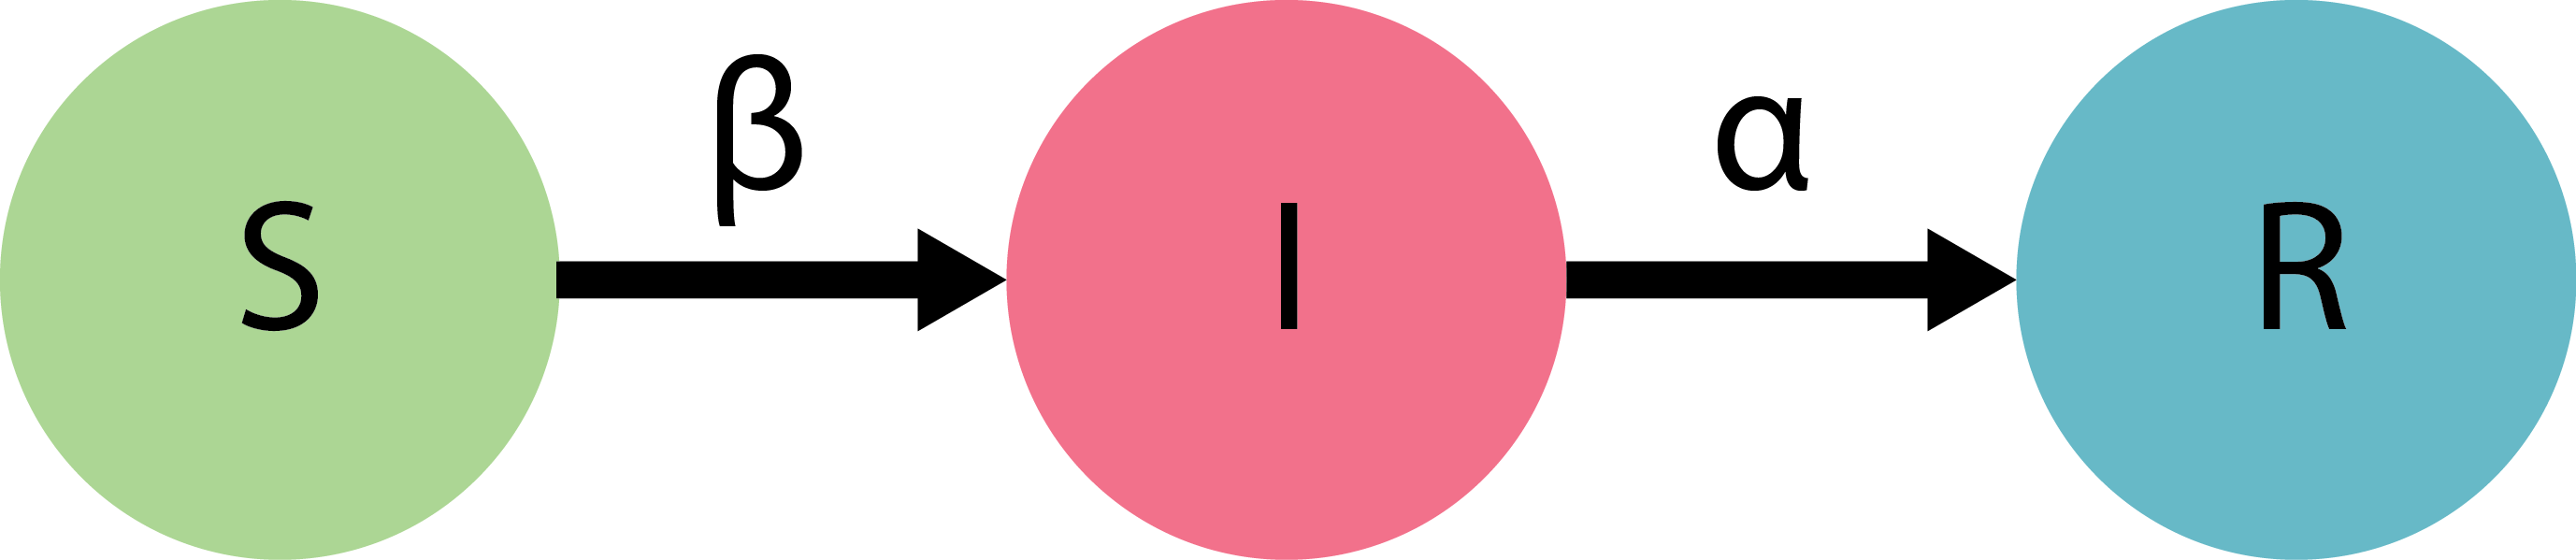
\includegraphics[width=\linewidth]{compartmental-models/SIR-compartments.png}
	\caption{Flowchart of the Kermack–McKendrick SIR epidemic model. The circles represent the compartments and the arrows show allowed transfers between them with the associated parameters of transfer rates above.}
\end{figure}
\\
Eq. (\ref{SIR1}) is justified by noting that the infection rate is positively correlated to the number of contacts between $S$ and $I$. We then use the law of mass action from assumption \ref{SIR-as-ma} to say that the number of contacts between infectives and susceptibles is proportional to the product of the size of the two interacting classes, $SI$. Introducing a proportionality constant $\beta>0$, we can say that $\beta SI$ individuals are infected per unit time. Here $\beta$ denotes the \textit{transmission rate}\footnote{Note there are different ways of defining $\beta$ that lead to a different dynamical system. The other popular way is to define $\beta$ in a way that leads to $\dot S=-\frac{\beta S I}{N}$. This has some potential benefits but it obscures the pedagogy.}. $\beta$ is a parameter that is the product of how often contacts between susceptible and infective individuals occur, $c$, and the probability that a contact leads to infection, $p$.\\
\\
Eq. (\ref{SIR3}) is found by assuming that the number of individuals getting better is proportional to the amount of individuals who are ill. We let $\alpha>0$ be the proportionality constant. This in effect assumes that the infective period has an exponential distribution\footnote{Let $u(s)=$ number of infective individuals at time $s$ after having been infective. Then $\dot u=-\alpha u\implies u(s)=u(0)e^{-\alpha s}$}.  This is the \textit{transition (or removal) rate}, the rate that infective individuals are removed by either recovery and immunisation or death. Equivalently, it  means that the time of infectivity is exponentially distributed with mean $1/\alpha$.\\
\\
Finally, assumption \ref{SIR-as-pop} tells us that Eq. (\ref{SIR2}) is determined by the other two equations. Also, if we included any removed individuals at the start of system, they would play no part in the dynamics. So without loss of generality, we can assume $R_0=0$ in the initial conditions.
\subsection{Analysing the model}
Whilst it is possible to derive exact analytical solutions to this system\cite{exact-SIR}, it is simpler and far more instructive to explore the qualitative behaviour and derive some important quantitative properties.\\
\\
Note that $R$ plays no role in the equations of $\dot S$ or $\dot I$. Therefore we can consider just these two coupled equations\cite{martcheva}. If we need $R$ we can easily get it back by using assumption \ref{SIR-as-pop} that $R=N-S-I$. Decoupling $R$ gives the 2-dimensional system:
\begin{eqnarray}
	\dot S=-\beta S I\label{red-SIR1}\\
	\dot I=\beta S I-\alpha I=(\beta S-\alpha)I\label{red-SIR2}
\end{eqnarray}
with initial conditions: $S(0)=S_0,I(0)=I_0, S_0+I_0=N$.
%\paragraph{Basic Dynamics}
\begin{figure}
	\centering
	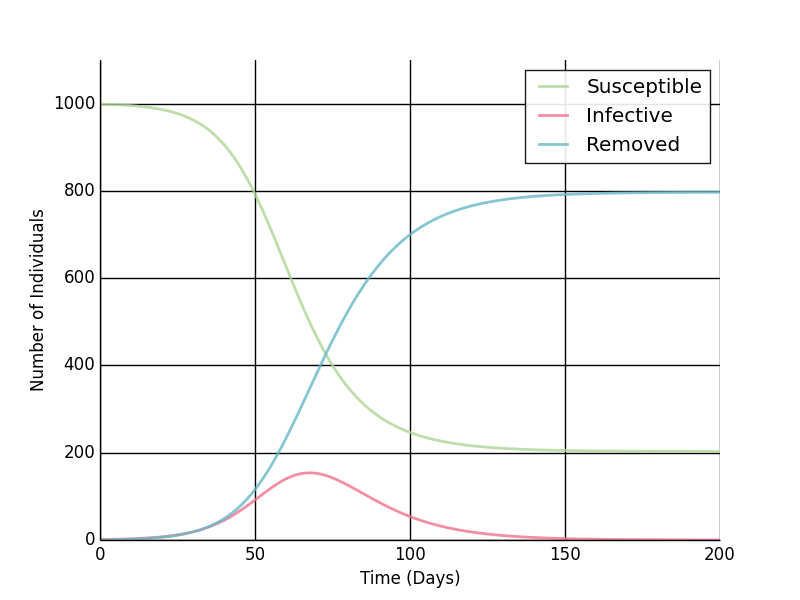
\includegraphics[width=1\linewidth]{compartmental-models/SIR-trajectory-fill.png}
	\caption{A typical SIR trajectory with $\beta=2\times10^{-3},\alpha=1/10, N=1000$}
\end{figure}
\subsubsection{Important quantities for epidemiologists}
Imagine you are the president of a country experiencing a significant epidemic. You have assembled a room full of leading epidemiologists to brief you. What do you ask them?
\subsubsection{Basic reproduction number, $R_0$}
Perhaps the first thing you will ask is: is the epidemic getting better or is it getting worse?\\
\\
As $\beta,S,I\geq 0$ it is immediate from Eq. (\ref{red-SIR1}) that $\dot S(t)=-\beta SI\leq 0$ for all $t$. That is the number of susceptibles is a decreasing function. Indeed if $S,I>0$ then it is strictly decreasing. So the number of susceptibles decreases until there are either no susceptibles or no infectives.\\
\\
Also, we have \[\dot I=(\beta S-\alpha)I>0\iff\beta S-\alpha>0\iff S>\alpha/\beta\] So $I$ increases only if $S>\alpha/\beta$. If $S_0<\alpha/\beta$, $I$ decreases for all $t$ and the infection dies without any increase in infection cases. Alternatively if $S_0<\alpha/\beta$, $I$ begins by increasing. But as established, $S$ is strictly decreasing for $I\neq0$ so $S$ decreases until eventually $S=\alpha/\beta$. At this point $I$ will reach a maximum. For all $t$ after this it will decrease to the limit $I=0$.\\
\\
From the arguments above $\beta S-\alpha$ plays a key role in the dynamics. We define the basic reproduction number $R_0=\beta S_0/\alpha$\cite{models-epidemiology-2}. Note that if $R_0>1$ the number of infective individuals will increase at time $t=0$. In this case we say that there is an epidemic. If $R_0\leq1$ the infection dies out without any increase in the number of infected individuals at any point.\\
\\
There is some disagreement among biologists and mathematicians over the exact definition and interpretation of $R_0$\cite{Heffernan281}. However, most models assume that $S_0\approx N$. This can be motivated by considering how an epidemic can begin. We can imagine a member getting infected through travel for example and returning to the population. Then $I_0=1$ and $S_0=N-1$. As we usually consider $N\gg1$ we have $S_0\approx N$. This assumptions allows us to consider $R_0$ as the number of infections passed on by a single infective individual during their infective period in a completely susceptible population.\label{mm}\\
\\
%Intuitively, $\beta S_0/\alpha$ is the number of infections passed on by a single infective individual during their infective period in the initial population.
%\textit{Mark's note- The population doesn’t need to be completely susceptible, does it? That would amount to defining $R_0$ as $R_0 = \beta N / \alpha$.}
%As models usually assume that $S_0\approx N$, it can also be considered as the number of infections passed on by a single infective individual during their infective period in a completely susceptible population\cite{models-epidemiology-2}.
This interpretation is easily understood. $\beta S$ is the rate of new infections caused by infections caused by a single infective individual. The mean length of an infective period is $1/\alpha$ by the assumption of exponentially distributed infections lengths. If an infected individual is, on average, not able to pass it on to at least one other person clearly the the infection will die out.
\subsubsection{Final size relation}
The next question you, as President, may ask is: how many people will the epidemic affect? This is given by the final size relation, an equation relating the number of affected individuals to $R_0$. Recalling that $\dot S\rightarrow0$ as $t\rightarrow0$, we can define $\lim_{t\rightarrow\infty}S(t)=S_\infty$. The number of individuals affected by the epidemic is the total number of individuals who have been infected at \textit{any} point. That is equal the size of the population minus the still susceptible population: $N-S_\infty$\label{mmd}. It can be shown that\cite{models-epidemiology} \[N-S_\infty=\frac{N}{R_0}\log(\frac{S_0}{S_\infty})\]
This is often written in the form \[\log(\frac{S_0}{S_\infty})=R_0(1-\frac{S_\infty}{N})\]\label{mmd} and called the \textit{final size relation}.
\subsubsection{Important quantities for revolutions}
The final size relation is an important quantity when studying infectious diseases because we care about the total number of affected individuals \textit{throughout} the diseases spread. However, in models of political revolutions it is of limited relevance. Instead we are interested in the amount of people active in sharing an idea at a single \textit{instant}. Instead of the epidemiological-minded \textit{final} size relation, we want a \textit{maximum} size relation. This would give a way of relating $R_0$ to the maximum size of the infective class $I_{\max}=\sup_{t\geq0}I(t)$.\\
\\
Firstly, let the infectious disease be the idea of a specific anti-regime group or movement. Let $S$ be the class of people who have not heard of this specific movement or have not been so far convinced by it. $I$ is the class of people who are convinced and actively sharing the ideas and taking part in revolutionary actions. Finally $R$ is the class of people who have been jailed, injured, fled the country or otherwise given up on actively supporting the cause.\\
%MM expand and slow down from here on out
\\
We assume that a revolution is successful if the proportion of active revolutionaries in a population is greater than some threshold value $r$ at some point. Formally, it is successful if there exists $t$ such that ${I(t)}/{N}\geq r$. This assumption of a threshold, whilst perhaps seeming oversimplistic, is backed by research\cite{logic-non-violence}. Further, this research suggests that the percentage of a population needed for a successful revolution is surprisingly small: just $3.5\%$\cite{logic-non-violence}. Some revolutions far surpass this number with an estimated $16\%$ of the Tunisian population actively participating in civil resistance in 2010\cite{arab-spring-percent}. While the analysis of this paper will not depend on the exact value of $r$, we will often use these two values $r=0.035$ and $r=0.16$ to get some values out of the derived equations.\\
\\
%MM expand a bit
As discussed, if $R_0\leq 1$ then no epidemic occurs and $I$ is decreasing for all $t$. In this case $I_{\max}=I_0$. So we assume $R_0>1$. Therefore we have $S_0>\alpha/\beta$. We define $t'>0$ to be the time such that $\dot S(t')=0$. Then $S(t')=\alpha/\beta$. From the previous arguments, $I(t)$ is increasing for $t$ when $0 \leq t<t'$ and decreasing for $t$ when $t'\leq t$. So $I$ reaches its maximum at $t'$. Formally, we have $I_{\max}=I(t')$.\\
\\
In mathematical epidemiology there is a classical equation to describe the maximum value of the infected class throughout the epidemic\cite{martcheva}:
\begin{equation}\label{eqn:imax}
	I_{\max}=S_0+I_0-\frac{\alpha}{\beta}+\frac{\alpha}{\beta}\ln\left(\frac{\alpha}{\beta}\right)-\frac{\alpha}{\beta}\ln(S_0)
\end{equation}\label{mmd}
This is very useful in modelling disease. If one can calculate $I_{\max}$ for a disease in its early stages, one is able to tell when the number of infections will decline\cite{martcheva}. However, we can adapt it to revolutions further.
\subsubsection{Maximum size relation}
Eq. (\ref{eqn:imax}) defines a subset of 4-dimensional space in $I_0\times S_0\times\alpha\times\beta$ with each point either leading to a revolution or not. This number of variables is acceptable if we know the specific parameters and are using it to calculate a value of $I_{\max}$. However, we can reduce it down further to 1-dimensional space in $R_0$ to obtain a more analytical insight.
\begin{align*}
I_{\max}&=S_0+I_0+\frac{\alpha}{\beta}\left(\ln\left(\frac{\alpha}{\beta}\right)-\ln(S_0)-1\right)\tab &\text{from \ref{eqn:imax}}\\
&=S_0+I_0+\frac{\alpha}{\beta}\left(\ln\left(\frac{\alpha}{\beta S_0}\right)-1\right)\tab &\text{by log rules}\\
&=S_0+I_0+\frac{\alpha}{\beta}\left(\ln\left(\frac{1}{R_0}\right)-1\right)\tab &\text{as } R_0=\frac{\beta S_0}{\alpha}\\
&=N+\frac{\alpha}{\beta}\left(\ln\left(\frac{1}{R_0}\right)-1\right)\tab &\text{as }S_0+I_0=N\\
&=N+\frac{\alpha}{\beta}(-\ln(R_0)-1)\tab &\text{by log rules}
\end{align*}
Recalling that a revolution happens if $I_{\max}/N\geq r$, we divide through by $N$:
\begin{align*}
\frac{I_{\max}}{N}&=\frac{N}{N}+\frac{\alpha}{\beta N}(-\ln(R_0)-1)\\
&=1+\frac{\alpha}{\beta N}(-\ln(R_0)-1).
\end{align*}
This is now in 3D space $\alpha\times\beta\times R_0(\alpha,\beta,S_0)$. To reduce it further we need to make an assumption. We assume that $I_0\ll S_0$ and thus that $S_0\approx N$. This can be motivated by supposing that, as we did for interpreting $R_0$, the revolutionary idea or movement comes from an individual or very small group or alternatively comes from outside the population of $N$ individuals. This allows us to write $\alpha/(\beta N)\approx \alpha/(\beta S_0)=1/R_0$. Then we can write \[\frac{I_{\max}}{N}=1+\frac{1}{R_0}(-\ln(R_0)-1)\]
Finally with a small rearrangement, we have what we can baptise \textit{the maximum size relation}:
\begin{equation}\label{eq:max-size}
	\frac{I_{\max}}{N}=\frac{R_0-1-\ln(R_0)}{R_0}:=m(R_0)
\end{equation}
valid for $R_0\geq1$.\\
\\
Bringing this together, we say a revolution occurs if and only if \[m(R_0)=\frac{R_0-1-\ln(R_0)}{R_0}\geq r \text{ for a given } r\]
\begin{figure}
	\centering
	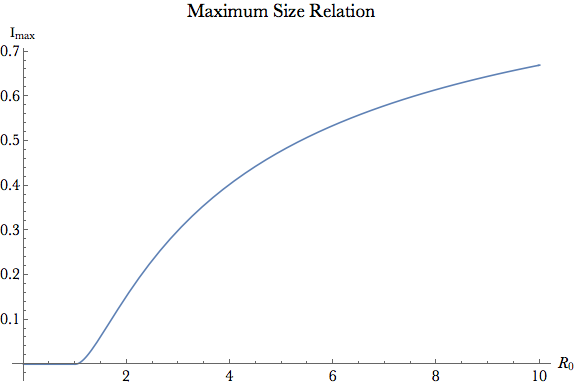
\includegraphics[width=0.95\linewidth, trim={0, 0 0 0.7cm}, clip]{/compartmental-models/maximum-size-relation.png}
	\caption{Graph showing how the maximum fraction of infectives in the population varies with the basic reproduction number $R_0$ in the SIR model. This is derived from the maximum size relation (Eq. (\ref{eq:max-size})). Note in particular how small values of $R_0$ can result in significant fractions of the population being active at the revolution's peak.}
\end{figure}
We can check that the proposed maximum size relation has desirable properties in relating $R_0$ to $I_{\max}/N$. The domain should be $R_0\geq 1$ as we excluded lower values in the derivation. Also as $I_{\max}/N$ is a proportion, we need to ensure that the codomain is restricted to $0\leq m(R_0) \leq 1$. We also presume that the higher $R_0$, the higher the value of $m(R_0)$. So to summarise this, we want an increasing function $m:[1,\infty]\rightarrow[0,1]$.\\
\\
It is increasing as \[\frac{d(I_{\max}/N)}{dR_0}=\frac{\ln R_0}{R_0^2}\geq0, \forall R_0\geq1\]
We also have $m(R_0=1)=0$. Further, as $R_0$ tends to infinity, $\lim_{R_0\rightarrow\infty}m(R_0)=1$\label{mmd}. As $m$ is an increasing function, these give the minimum and maximum respectively. So the proposed maximum size relation has all the desired properties.\\
\\
We can provide some intuition for the maximum size relation by interpreting the $\frac{R_0-1}{R_0}$ term as how much over the threshold of $1$ $R_0$ is. Clearly the larger it is, the higher we can expect $I_{\max}$ to be. However, this potentially unlimited growth is inhibited by the ${-\ln(R_0)}/{R_0}$ term, representing the depletion of the susceptible population and thus a reduction in transfer rate $\beta S I$.\\
\\
Note that this analysis holds for the SIR model in general and can be used to roughly predict the number of infective cases that will be occurring at an infection's peak severity. This is useful in telling when an epidemic will begin to decay away. However if a researcher was calculating $I_{\max}$ from the SIR model, they would find estimate values of $\alpha,\beta,S_0,I_0$ and calculate $I_{\max}$ from Eq. (\eqref{eqn:imax}). In practice they would not use the SIR model but instead base these calculations on a more specialised model. However, for our analytical purposes it is very useful. We can interpret $R_0$ as the amount of people the average revolutionary would have to convince to be part of their movement if no one in the population had yet heard of the movement.\\
\\
If we desire a quick estimate of some values, we can naively apply the SIR model to the study of revolutions. As discussed earlier, research suggests that the threshold is given by $r=0.035$. Using the freshly created maximum size relation we see that to get to the critical value of an engaged populace needed for a revolution we need a basic reproduction number of $R_0=1.338$ . In other words, each revolutionary must be able to, if in a fully susceptible population, convince $1.338$ people to join the revolution before they are removed. For the Tunisian revolution in 2010 with $16\%$ of the population involved in the revolution\cite{arab-spring-percent}, solving Eq. (\ref{eq:max-size}) yields $R_0=2.04$.\label{mmd} This is a basic reproduction number comparable to that of the relatively uninfective Ebola\cite{b-r-n}.
\section{SEIR Model}
A simple and instructive modification we can make to the SIR model is to add a new class. Many infectious diseases have a period in which an individual can be \textit{infected} but not yet \textit{infective}. We call this state being \textit{exposed}. In our revolutionary interpretation, exposed individuals are those who have heard and are convinced by the revolutionary idea but are not yet presenting as active. We can represent this in a compartmental model by adding the exposed class $E$ to the SIR model, creating the SEIR model. 
\begin{figure}[h]
	\centering
	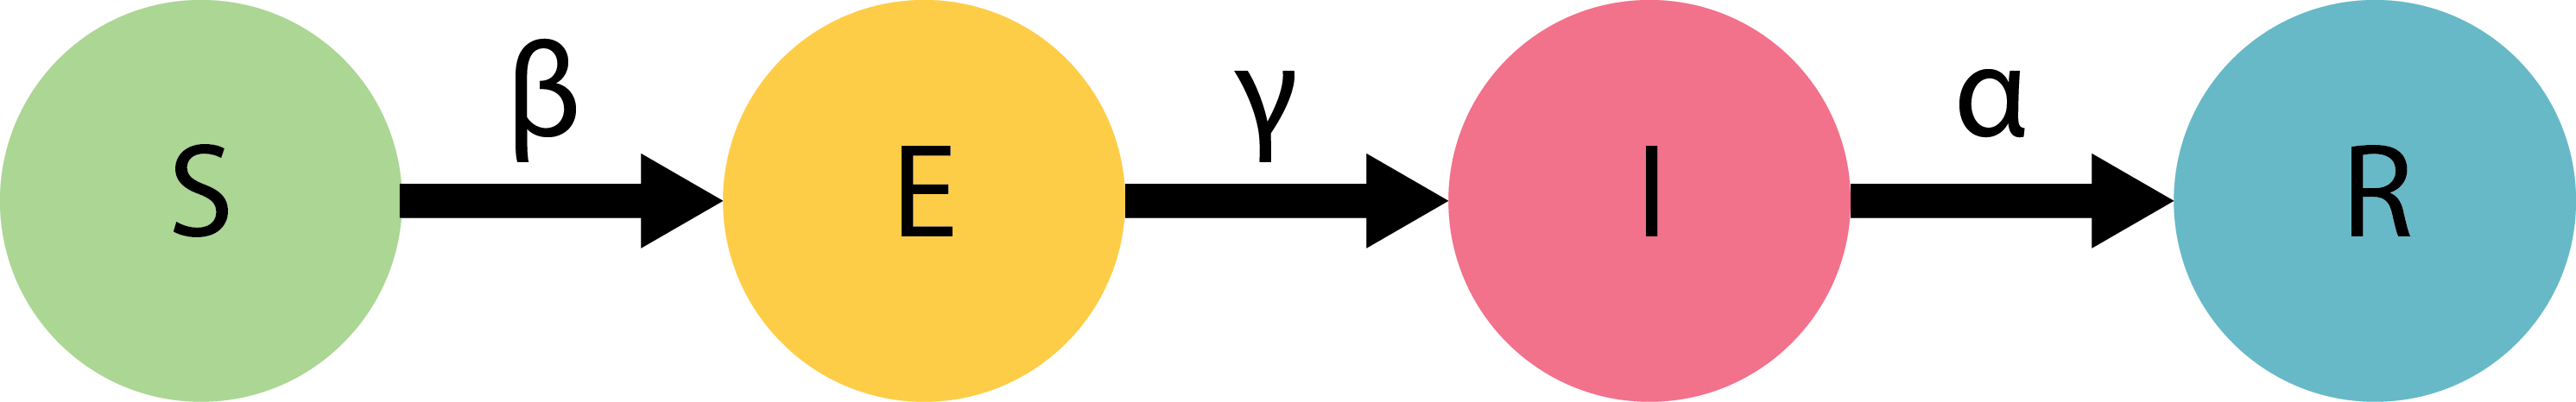
\includegraphics[width=\linewidth]{compartmental-models/SEIR-compartments.png}
	\caption{Flowchart of the SEIR epidemic model. Note that this is an extension of the SIR model that introduces an extra compartment $E$ and the transfer rate $\gamma$ between $E$ and $I$.}
\end{figure}

\subsection{Building the model}
We assume the exposed period is exponentially distributed with mean $1/\gamma$. Again this is equivalent to assuming that the rate of moving from $E$ to $I$ is proportional to the number of exposed individuals. This gives the dynamical system:\\
\begin{eqnarray}
\dot S=-\beta S I\\
\dot E=\beta S I-\gamma E\\
\dot I=\gamma E-\alpha I\\
\dot R=\alpha I
\end{eqnarray}
As before, we remove R to reduce the system by a dimension to give:\label{mmd}\\
\begin{eqnarray}
\dot S=-\beta S I\label{SEIR1}\\
\dot E=\beta S I-\gamma E\label{SEIR2}\\
\dot I=\gamma E-\alpha I\label{SEIR3}
\end{eqnarray}
\subsection{Analysing the model}
\begin{figure}
	\centering
	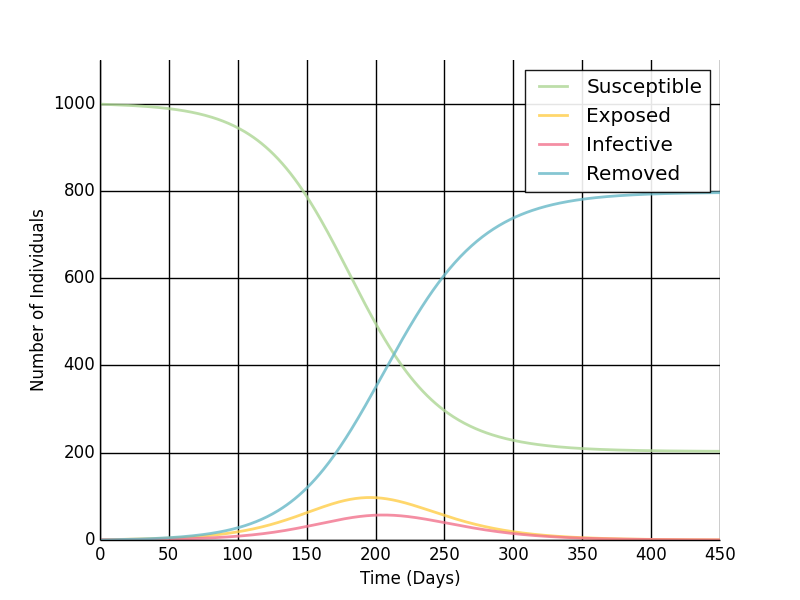
\includegraphics[width=\linewidth]{compartmental-models/SEIR-trajectory-fill.png}
	\caption{A typical SEIR trajectory with $\beta=3,\alpha=1/10,\gamma=1/300$}
\end{figure}
In the SIR model we could tell if an epidemic would occur simply by seeing if there was initial growth in the infective class. This worked because, if the infective class did not grow initially, it could not grow at any later time. However, the SEIR model is more complex and can have initial decline yet still see an epidemic. As we can no longer use our previous definition of an epidemic occurring we are motivated to develop a new, more general one.\\
\\
%Instead it is characterised by the equilibrium with all individuals of the population susceptible
One possibility is to consider the disease-free equilibrium (DFE). This is the equilibrium that occurs when the whole population is in the susceptible class. In the SEIR system (\ref{SEIR1}-\ref{SEIR3}) the DFE is given by $(S,E,I)=(N,0,0)$. It is easy to see that this is in fact an equilibrium in the SEIR system and gives $\dot S=\dot E=\dot I=0$. In fact in all reasonable deterministic epidemic models this is an equilibrium: if there is no-one with the infectious disease and no randomness in the model, there is no way for the disease to enter the population and so everyone will stay susceptible. So if no-one is infective with the disease no-one ever will be.\\
\\
We say that an epidemic occurs if a small divergence from the DFE results in the system moving away from the DFE. Otherwise if the system does not move further away from the DFE, we say no epidemic occurs. One way to motivate this is to consider what would happen if a small number of infectives were released into the population. If they are able to infect more people, an epidemic occurs and we move from the DFE. Otherwise, the number of infective individuals decreases until there are no more. Translating this into mathematics we say an epidemic occurs if the DFE is unstable and an epidemic does not occur if the DFE is asymptotically unstable \footnote{See Section \ref{dynamical-systems} for a primer on dynamical systems}\cite{models-epidemiology-2}.\label{aa}\\
\\
The stability of SEIR can be investigated by linearising about the DFE. To do this we calculate the Jacobian at the DFE, $\bf{x}^*=(N,0,0)$,\\
\[
\bf{J}_{(\bf{x}^*)}=
{\begin{bmatrix}
	{\partial \dot S \over \partial S} &
	{\partial \dot S \over \partial E} &
	{\partial \dot S \over \partial I} \cr 
	{\partial \dot E \over \partial S} & 
	{\partial \dot E \over \partial E} & 
	{\partial \dot E \over \partial I} \cr 
	{\partial \dot I \over \partial S} & 
	{\partial \dot I \over \partial E} & 
	{\partial \dot I \over \partial I}
\end{bmatrix}}
_{(\bf{x}^*)}
={\begin{bmatrix}
	{-\beta I} &
	{0} &
	{-\beta S} \cr 
	{-\beta I} & 
	{-\gamma} & 
	{\beta S} \cr 
	{0} & 
	{\gamma} & 
	{-\alpha}
	\end{bmatrix}}
_{(\bf{x}^*)}
={\begin{bmatrix}
	{0} &
	{0} &
	{-\beta N} \cr 
	{0} & 
	{-\gamma} & 
	{\beta N} \cr 
	{0} & 
	{\gamma} & 
	{-\alpha}
	\end{bmatrix}}
\]
\\
Then finding the eigenvalues we get the determinant and resulting characteristic equation
\[{\begin{vmatrix}
	{-\lambda} &
	{0} &
	{-\beta N} \cr 
	{0} & 
	{-\gamma-\lambda} & 
	{\beta N} \cr 
	{0} & 
	{\gamma} & 
	{-\alpha-\lambda}
	\end{vmatrix}}=-\lambda\big((-\gamma-\lambda)(-\alpha-\lambda)-\beta N\gamma \big)\]
So $\lambda=0$ is an eigenvalue. This corresponds to the line of equilibria in which $E=I=0$. This is the system in which every individual is either susceptible or removed.\label{mmd}\\
\\
The other eigenvalues are the eigenvalues of the matrix:
\[{\begin{vmatrix}
	{-\gamma} & 
	{\beta N} \cr 
	{\gamma} & 
	{-\alpha}
	\end{vmatrix}}\]
These have negative real part if and only if the determinant of the matrix is positive\cite{models-epidemiology-2}. The determinant $\gamma(\alpha-\beta N)$ is positive if and only if $R_0<1$. Note that the trace of the matrix is negative and so the negative eigenvalues correspond to the stability of the equilibrium and the failure of an epidemic to develop\cite{models-epidemiology-2}. Hence again, the stability of the equilibrium in the SEIR model again depends on if $R_0$ is greater or less than $1$.

%This has determinant $\gamma(\alpha-\beta N)$. As $\gamma>0$, the determinant is positive if and only if $\alpha-\beta N$ is positive which is equivalent to $R_0<1$. An equilibrium point is unstable if there exists an eigenvalue with positive real part. We also know that a matrix's eigenvalues have negative real part if and only if the determinant is positive. And so if $R_0<1$, the DFE is stable. Otherwise it is unstable. \label{aa}
%\textit{Mark's note: Your claim about the value of the determinant and the signs of the real parts of the eigenvalues is too strong and actually false for matrices of odd dimension. The simplest way to fix this is to say something like:
%“The eigenvalues of a two-by-two matrix may have negative real part only if the determinant is positive”.}
\label{mmd}
\section{Model of revolution}\label{sec:rev-compartment}
%We can adapt the SEIR model to make an explicit compartmental model of revolution. A natural question is to consider if the basic flow should be the same. \label{mmd}
\subsection{Building the model}
% need a bit introducing E and also the analogy explicitly.
% also should I change the names of the compartments? Or does that make it more complicated?
The intrinsic difference between the spread of an infection and the spread of an idea is an individual's agency. With a general idea, this agency is not particularly important and can be bundled up with the transmission rate $\beta$. This parameter $\beta$ tells us about the average individuals likelihood of spreading an idea. However, with a revolutionary idea this agency is intrinsic. Most people who hold a revolutionary idea do not only consider the idea and see if they want to share it. They will also check the surrounding environment to see if others are sharing the idea, what the danger to them is and what the likelihood of a successful revolution is. To account for this we need an activation rate that is a function of the population demographic.\\
\\
Specifically, exposed individuals who are thinking about becoming active revolutionaries will look at what percentage of the population are already active revolutionaries. This is given by $I/N$. Fellow exposed individuals are invisible as they are not making any actions that display their support for a revolution. So we want the activation rate to be a function solely of $I/N$. So far, we do not know the nature of this function. For now we denote it $g(x):[0,1]\rightarrow\mathbb{R}$.\\
\\
Given the context it is natural to wonder if our model should allow transfers from $E\rightarrow R$. This corresponds to people who became convinced that the revolution is desirable but have since gone off the idea without ever having become revolutionaries. Whilst this is certainly possible it turns out that this is neither conceptually nor mathematically necessary. Conceptually, an exposed individual, while exposed has no effect on the wider population, much like a removed individual. In particular, they do not contribute to the size of the infective class which is the value we care most about. As the outwards effect on the dynamics between exposed and removed is negligible, an exposed individuals change to removed has no outward effect on the dynamics. Mathematically, we can account for this by making the value we give for $N$ smaller by a fraction corresponding to the fraction of people we expect to move directly from exposed to removed.\label{mmd}
\begin{figure}[h]
	\centering
	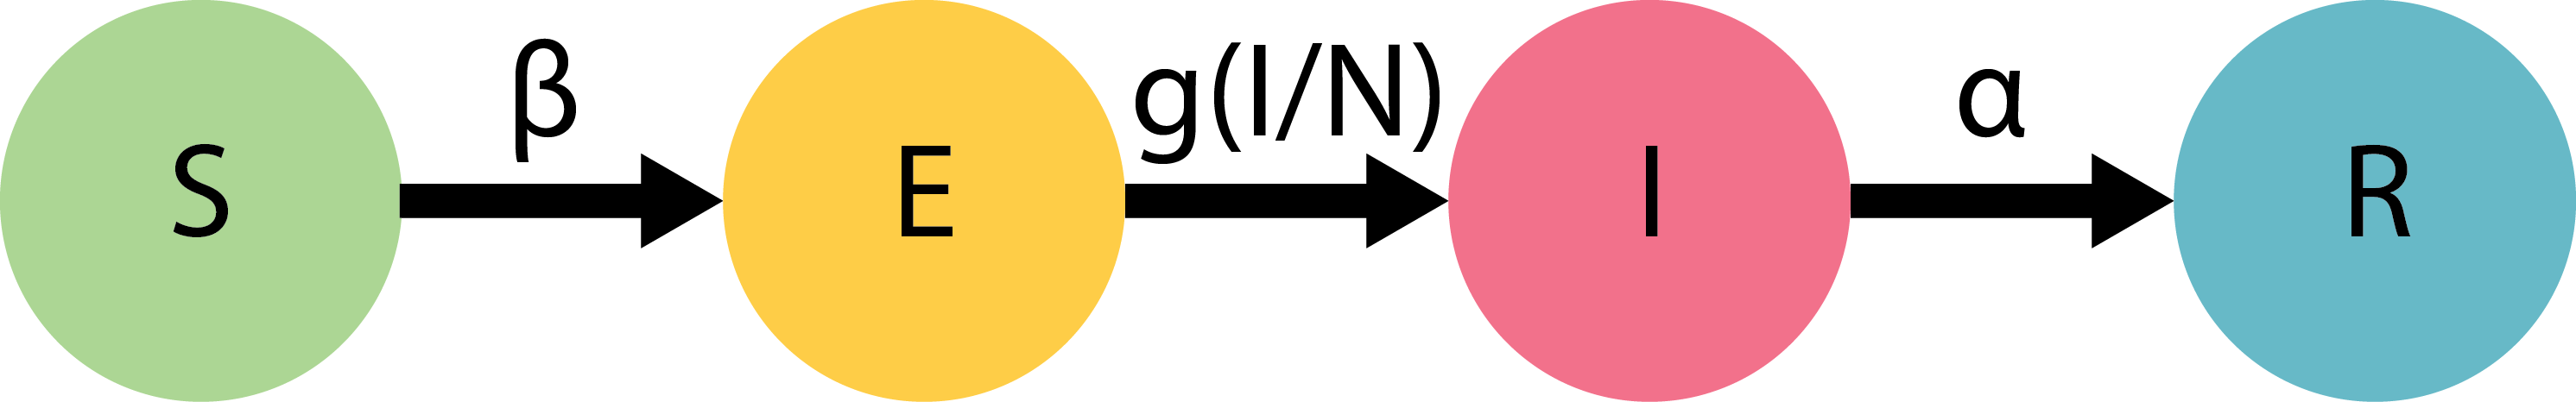
\includegraphics[width=\linewidth]{compartmental-models/rev-compartments.png}
	\caption{Flowchart of the compartmental model of revolution}
\end{figure}\\
\\
Adapting the SEIR model but allowing potential non-linear movement between the exposed and infective compartments, we get a dynamical system:
\begin{eqnarray}
\dot S=-\beta S I\\
\dot E=\beta S I- \gamma E g(I/N)\\
\dot I= \gamma E g(I/N)-\alpha I\\
\dot R=\alpha I
\end{eqnarray}
where $g(x)$ is the as yet unknown function.
\subsubsection{In search of $g(x)$: a naive approach}
The dynamics of collective behaviour are complex but there are some findings that are well-supported. People's proclivity towards behaving in a certain way often depends on how many people are already behaving that way. One of the dominant models of this in social psychology has been the threshold model. This holds that we tend to act in a certain way only if a certain number of other individuals are acting in that way\cite{threshold-models-social-influence}.\\
\\
Let $k$ be some threshold value with $0\leq k\leq1$. Then one option is to adapt the function from Granovetter's original paper on threshold models from absolute numbers of people to proportions of people. This would mean we have a discontinuous step function:\\
	\[
g_1(x) = \left\{\begin{array}{lr}
1, & \text{if } x\geq k\\
0, & \text{if } x< k
\end{array}\right\}
\]
where $k$ represents the threshold.\\
\\
A continuous alternative is given by:
\[g_2(x)=\frac{x^n}{k^n + x^n}\]
\begin{figure}
	\centering
	\begin{subfigure}{.46\textwidth}
		\centering
		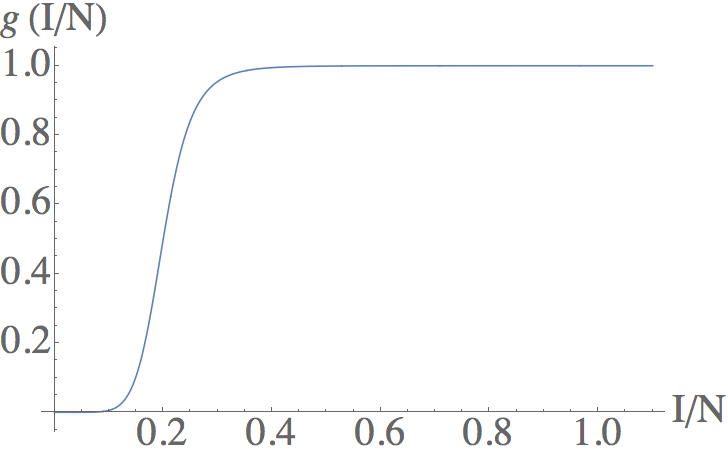
\includegraphics[width=\linewidth]{compartmental-models/rev-transfer-rate1.png}
		\caption{$n=2$}
	\end{subfigure}%
	\begin{subfigure}{.46\textwidth}
		\centering
		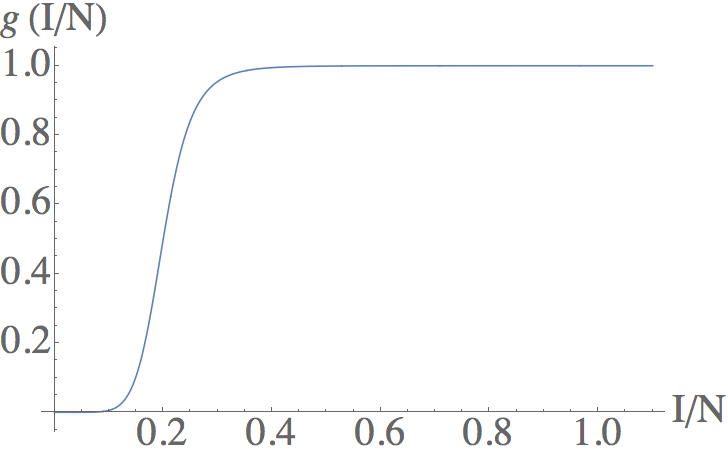
\includegraphics[width=\linewidth]{compartmental-models/rev-transfer-rate2.png}
		\caption{$n=7.5$}
	\end{subfigure}
	\begin{subfigure}{.46\textwidth}
		\centering
		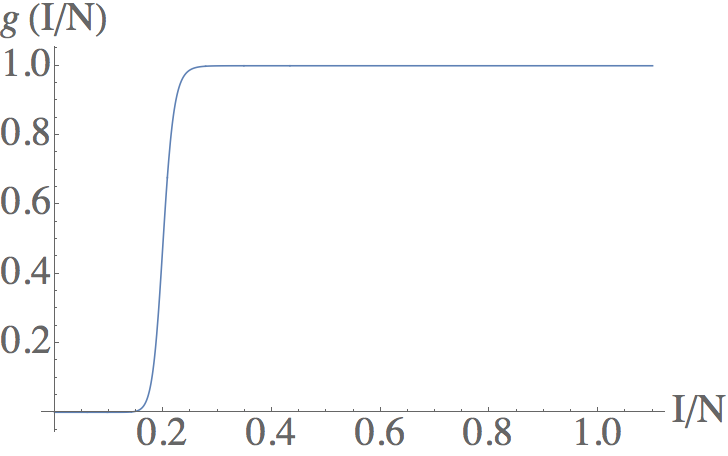
\includegraphics[width=\linewidth]{compartmental-models/rev-transfer-rate3.png}
		\caption{$n=20$}
	\end{subfigure}
	\caption{The effect of different values of $n$ on the transfer rate $g_2(x)$ with $k=0.2$.}
	\label{fig:transfer-rate-n}
\end{figure}
Here $k$ controls the threshold value with $g_2(x)={1\over2}$ at $x=k$. $n$ controls the severity of the threshold with a higher $n$ giving a steeper curve and a more sudden phase change. $g_2$ is preferable to $g_1$ both practically and theoretically. Practically, the continuity allows us to analyse the function at all points of the domain using standard calculus. Theoretically, it better represents the non-uniformity of a population's attitude to risk and the fuzzy boundary around giving an \textit{exact} threshold for active participation.\\
\\
We allow the possibility of scaling by a factor $\gamma$. Then $\gamma g(I/N)$ is the probability that an exposed individual will become active in one unit time. So if $I/N\approx1$, the probability of an exposed individual becoming active per unit time is roughly $\gamma$. This gives the number of individuals leaving $E$ per unit time as $\gamma Eg_2(I/N)$. So we have the dynamical system:
\begin{eqnarray}
\dot S=-\beta S I\\
\dot E=\beta S I- \gamma E \frac{(I/N)^n}{k^n + (I/N)^n}\\
\dot I= \gamma E \frac{(I/N)^n}{k^n + (I/N)^n}-\alpha I\\
\dot R=\alpha I\label{rev1eq4}
\end{eqnarray}
\subsubsection{Finding suitable parameters}
There are now 6 parameters in our model. We justify the default values used in Table \ref{tab:parameters1}. Unless otherwise stated, all simulations and graphs will use the values of the parameters as given in this table. For the initial conditions we start with a single revolutionary giving $I_0=1$ and $S_0=N-1$.
\begin{table}
	\captionof{table}{Default Parameter Values} \label{tab:parameters1} 
	\centering
	\begin{tabular}{| l | l | p{7.5cm} |}
		\hline
		Parameter (units) & Chosen Value & Justification \\ \hline
		N (people) & 2 million & $1/5$ of the population of Tunisia in 2010 (10.6 million). This is an estimate of how many people were potentially open to protesting (based on political orientation, age, medical history etc.).\\ \hline
		$\alpha$ (1/days) & 1/300 & Noting the exponential distribution inferred by Eq. (\ref{rev1eq4}), this assumes that a protester is removed through some means, on average, after 300 days of protesting. \\ \hline
%		$\beta$ (1/days$\cdot$people) & $2.04\cdot \alpha/N$ & Using $\alpha,N$ and the value of $R_0=2.04$ we calculated for the Tunisian revolution using the maximum size relation we get $\beta\approx\alpha R_0/N$. \\ \hline
		$\beta$ (1/days$\cdot$people) & $40\cdot \alpha/N$ & We assume that a revolutionary could expose around $50$ people to the idea in a completely susceptible population. Using the basic reproduction number we have $\beta\approx\alpha R_0/N$. \\ \hline
		$\gamma$ (1/days) & 1/5 & If conditions are right, it takes $5$ days on average for someone to move from exposed to active. \\ \hline
		$n$ (dimensionless) & 3 & This corresponds to a slightly steep curve of $g(x)$. \\ \hline
		$k$ (dimensionless) & 3/50 & The Asch conformity experiments found that an individual is highly influenced by 3 people to act in a way so as to conform with them\cite{asch-conformity}. However, increases to four and beyond have little effect. We assume each person is influenced by around $50$ people. \\ \hline
		$\delta$ (days) & $\gamma/200=1/1000$ & 
		We guess that around one in every 200 people is a potential `zealot'. If conditions are right, there are $1/\gamma$ people converting to active each unit time because of observing the population. There are 1/200 of the population converting who would have converted regardless of the political situation. \\ \hline
	\end{tabular}
\label{tab:parameters-compartments-1}
\end{table}

\subsubsection{Results and failure of the naive approach}
To keep things clean, we write \[\theta(I)=\frac{\partial g_2(I/N)}{\partial I}=\frac{k^n n (I/N)^n}{I(k^n+(I/N)^n)^2}\]
Decoupling $R$ as before, the Jacobian at the DFE
\[
\bf{J}_{(\bf{x}^*)}
={\begin{bmatrix}
	{-\beta I} &
	{0} &
	{-\beta S} \cr 
	{-\beta I} & 
	{-\gamma g_2(I/N)} & 
	{\beta S-\gamma E\theta(I)} \cr 
	{0} & 
	{\theta g_2(I/N)} & 
	{\gamma E \theta(I)-\alpha}
	\end{bmatrix}}
_{(\bf{x}^*)}
={\begin{bmatrix}
	{0} &
	{0} &
	{-\beta N} \cr 
	{0} & 
	{0} & 
	{\beta N} \cr 
	{0} & 
	{0} & 
	{-\alpha}
	\end{bmatrix}}
\] 
The resulting zero eigenvalues mean that we cannot ascertain whether it is a stable equilibrium. So we have to get creative. We could look at the Hessian, the square matrix of second order partial derivatives. However, this is a $9\times9$ matrix and we now have 6 parameters so this is neither fun nor informative. Instead we go exploring.\\
\\
The fact that there are zero eigenvalues suggests that the DFE is in fact part of an infinite number of equilibrium points. From observation, we can see that $(S^*,E^*,0)$ are all equilibrium points. These are the equilibriums in which there are varying degrees of revolutionary powder but no spark.\\
\\
To have an increase in the number of infectives we need the number of invididuals becoming infective to be greater than the number of those ceasing to be infective. Noting that $g_2(x)$ behaves like $n(\frac{x}{k})^n$ for small perturbations $x$ from $0$
\footnote{$g_2(x)$ has a Taylor expansion about $0$ of
\[g_2(x)=0+\frac{nk^nx^{n-1}}{(k^n+x^n)^2}\cdot x+...\approx \frac{nk^nx^{n}}{(k^n+x^n)^2}\] Noting that a small perturbation $x$ is much less than the threshold value $k$ we have $x\ll k$. Hence $k^n+x^n$ is dominated by the $k$ term. This gives the formula \[g_2(x)\approx\frac{nk^nx^n}{(k^n)^2}=\frac{nk^nx^{n}}{k^{2n}}=n\left(\frac{x}{k}\right)^n\]}. Therefore to have an increase in infectives we require that:
\begin{alignat}{2}
\gamma E n &\left( \frac{I/N}{k} \right)^n &&> \hspace{1.5em}\alpha I\label{eq:gamma-1}\\
&\hspace{1em}\gamma &&> \sqrt[n]{\frac{\alpha I}{E n}}k\frac{N}{I}\label{eq:gamma-2}
\end{alignat}
We know that $E<N$ and also that for $I$ to grow Eq. (\ref{eq:gamma-2}) must hold initially at $t=0$. So we can require $I=I_0=1$. Making these substitutions gives the requirement that
\begin{align*}
\gamma >& \sqrt[n]{\frac{\alpha}{N n}}k N
\end{align*}
If we use the default values to solve for $\gamma$, Eq. (\ref{eq:gamma-2}) gives a requirement that $\gamma>386$. This means that, on average, individuals become active less than $1/386$ of a day after having been exposed to the revolutionary idea. That is equal to four minutes which is barely enough to time to finish your cuppa.\\
\\
Therefore, we assume that with reasonable parameters the number of infectives is decreasing. So the only change can be that the active revolutionary dies and maybe some people become exposed to the idea. As we have $I_0=1$, the number of people who will be exposed is approximately equal to the number of people the active revolutionary can inform. That is exactly $R_0=\beta N/\alpha$.\\
\\
So we expect for any reasonable values, introducing a single revolutionary into the system will result in $I\rightarrow0$ as $t\rightarrow\infty$ while $E\rightarrow R_0$. This is in fact exactly what happens. With default parameters $R_0=2.04$ and so the revolutionary exposes two people to the idea before being snuffed out. Using a high value of $\beta$ as in Fig. \ref{fig:rev-naive-beta-high} we can visually see the system coming to its equilibrium point $(S^*,E^*,0)=(N-R_0,R_0,0)$.
\begin{figure}[!h]
	\centering
	\begin{subfigure}{0.8\textwidth}
	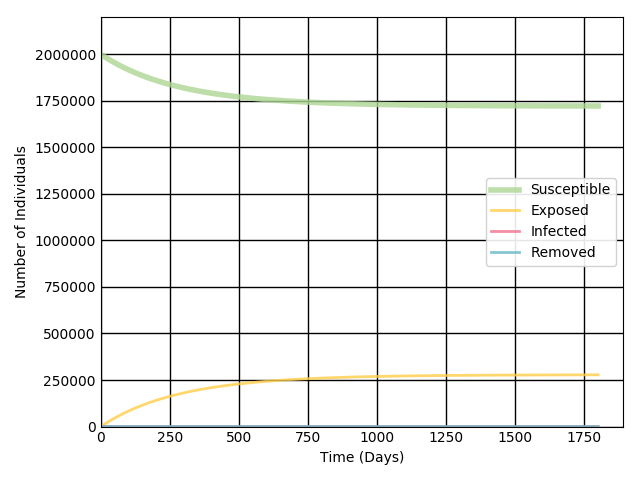
\includegraphics[width=\linewidth]{compartmental-models/failure-naive-approach3.png}
	\caption{A high, but still humanly possible, value of $\beta=1000/N$. This corresponds to each revolutionary exposing $1,000$ people a day to the revolutionary idea.}
	\label{fig:rev-naive-beta-high}
	\end{subfigure}
	\begin{subfigure}{0.8\textwidth}
		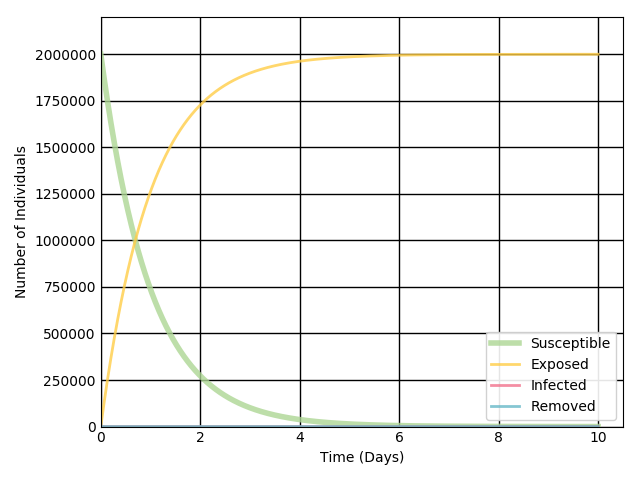
\includegraphics[width=\linewidth]{compartmental-models/failure-naive-approach2.png}
		\caption{A superhuman value of $\beta=1$. This corresponds to a revolutionary exposing roughly $1,000,000$ people to the revolutionary idea in a day.}
		\label{fig:rev-naive-beta-vhigh}
	\end{subfigure}
\caption{The compartmental revolution model with default parameters and high values of $\beta$. The resulting figures show the problems with the naive approach to the transfer rate $g(x)$.}
\end{figure}
\\
\\
Even if the active revolutionary is supernaturally effective, able to convince millions of people each day of the need for a revolution, he still suffers the same fate: dying whilst no other individual becomes active. This would involve having an unusually high transmission rate $\beta$. We set $\beta=1$, more than a million times the default parameter (Fig. \ref{fig:rev-naive-beta-vhigh}). Within two days we merely end up with the whole population convinced that they $\textit{should}$ do something. Meanwhile, the lonely active revolutionary becomes half a person, a third, reducing in size until he is infinitesimal. There is a powder keg of two million people but the only spark was left to die. Unfortunately, an idea without action remains just an idea.
%
\begin{tcolorbox}
	\paragraph{Lesson for revolutionaries:} An idea alone will never cause outward action. You must act in line with your beliefs to show others \textit{what} you believe. Otherwise everyone can believe in change yet do nothing about it.
\end{tcolorbox}
So in this model the most the revolutionary can hope for is to inform a lot of people that there \textit{should} be a revolution. Due to a limit on how quickly people move from being convinced of something to acting on it, there can never be an increase in the number of active revolutionaries.  This is a fatal problem for a model of revolution.\\
\\
Intuitively what has gone wrong is that when there is only one lone revolutionary, it's not particularly tempting to join them. The threshold model we have incorporated reflects the truth that most people do not want to be trend-starters. Most people, for better or worse, are sheep. However, fortunately change is possible. \textit{Most} people is not \textit{all} people.
\subsubsection{Improving $g(x)$: Thank God for the Zealots!}\label{sssec:zealots}
Some proportion of every society are zealots. They are the ones who are not afraid to stick their head above the pulpit. The fact that no one else is doing it does not faze them. In fact, they might actively enjoy it. These are the people who, upon hearing an idea they agree with, do not check to see if others hold and are expressing the idea. They simply express the idea. To get ourselves out of our rut, we assume that some proportion of the population are zealots.\\
\\
One option would be to introduce zealots as a category, with the majority of the population taking the traditional route route $S\rightarrow E\rightarrow I\rightarrow R$ and zealots perhaps moving directly $S\rightarrow I\rightarrow R$. However an alternative is to adopt this fraction of the population into the transfer rate $g$. This allows us to keep much of the analysis from the SEIR model.
%\textit{ Mark's note: This seems a good idea, but perhaps you should introduce zealots as a separate category of person who progress S -> I -> Rand then have the E -> I process depend on the sum of the population of ordinary Exposed people and the Infective Zealots.}
\label{mmd}
Then we choose instead \[g_3(x)=\delta+\gamma\frac{x^n}{k^n + x^n}\]
Note that this absorbs $\gamma$ into $g(x)$ so that it does not interfere with $\delta$. We can calculate a value of $\delta$ from imagining the transfer from $E$ to $I$ when the proportion of infectives $I/N$ is well past the threshold $k$. Then ${x^n}/({k^n + x^n})\approx1$ and the number of `ordinary' people per unit time who look at the population before deciding to be active is $\sim\gamma$. That is $\gamma$ people are converting for these reasons when the revolution is flowing per unit time. Similarly, $\delta$ people per unit time convert as `zealots' to the cause for reasons unrelated to the state of the revolution. Then we have have that the proportion of zealots in the initial population is given by $\delta/{(\delta+\gamma)}$\footnote{$\frac{\# \text{ zealots}}{\# \text{ individuals}}=\frac{\# \text{ zealots}}{\# \text{ zealots}+\# \text{ non-zealots}}=\frac{\delta}{\delta+\gamma}
%	=\frac{\gamma}{\delta+\gamma}$
$
}.
This gives us a way to find a meaningful value of $\delta$ (Table \ref{tab:parameters-compartments-1}).\\
\\
With this adoption the change in $E$ per unit time is given by:
\begin{equation*}\label{eq:g_3}
Eg_3(I/N)=E\cdot \big(\delta + \gamma\frac{(I/N)^n}{k^n + (I/N)^n}\big)
\end{equation*}
We can justify this term. The number of conversions to activity is proportional to the number of exposed individuals $E$. The first term in the brackets, $\delta$, represents those who, upon hearing an idea they agree with, become active regardless of the situation. The second term in the brackets $\gamma {(I/N)^n}/({k^n + (I/N)^n})$ represents the others who do a calculation by looking at what percentage of the population is active.\\
\\
It is worth noting that the value of $\delta$ is calculated using the fraction of zealots in the initial population. However this fraction changes as zealots are leaving the susceptible population at a different rate to the non-zealots in general this proportion will change during the revolution. This divergence is potentially a problem and difficult to justify analytically. However in practice, given the parameter values we use in the simulation, it has a negligible effect. Mathematically, the number of zealots who have become infective by time $t$ is $\int_0^t E\delta dt$. We will see in the model that in the early stages when zealots play the key role, $\int_0^t E\delta dt$ is very small compared to $N$ and so only a small amount of the total zealots have left the population.
%Similarly, the total number of individuals who have become infective is $\int_0^t Eg_3(I/N) dt$.
%Therefore, the fraction of the susceptible population that are zealots after time $t$ is at least as big as \[\frac{\delta}{\delta+\gamma}-\frac{\int_0^t E\delta dt}{N}\]
%in a population $\delta/{(\delta+\gamma)}$ should be altered by a factor that is at least close to $1$ as ${(N-\int_0^t E\delta dt)}/{N}$.
%So the effect of depleting zealots is only significant if $\int_0^t E\delta dt$ is comparable to $N$. We will return to see if this is the case in the simulations.
\label{mm}
\\
\\
Using $g_3$ results in the dynamical system:
\begin{eqnarray}
\dot S=-\beta S I\\
\dot E=\beta S I- E \left(\delta + \gamma\frac{(I/N)^n}{k^n + (I/N)^n}\right)\\
\dot I= E \left(\delta + \gamma\frac{(I/N)^n}{k^n + (I/N)^n}\right)-\alpha I\\
\dot R=\alpha I
\end{eqnarray}

\subsection{Analysing the model}
\subsubsection{Analytic results}
Reducing to three dimensions as before, the Jacobian at the DFE
$\bf{x}^*=(N,0,0)$ is\\
\[
\bf{J}_{(\bf{x}^*)}
={\begin{bmatrix}
	{-\beta I} &
	{0} &
	{-\beta S} \cr 
	{-\beta I} & 
	{-\delta-\gamma g_3(I/N)} & 
	{\beta S} \cr 
	{0} & 
	{\delta+\gamma g_3(I/N)} & 
	{-\alpha}
	\end{bmatrix}}
_{(\bf{x}^*)}
={\begin{bmatrix}
	{0} &
	{0} &
	{-\beta N} \cr 
	{0} & 
	{-\delta} & 
	{\beta N} \cr 
	{0} & 
	{\delta} & 
	{-\alpha}
	\end{bmatrix}}
\]
The addition of the `zealots' term makes the stability conditions of the revolution model reduce  to the conditions for the SEIR model. So by the arguments there, for a small disturbance from the DFE, there is no epidemic if $R_0<1$. However, from this we do not know how large the active population will grow. Further, it does not say anything about a large disturbance $I_0>0$ such that the non-zealot population becomes significant. To understand some of these details we need to create a simulation of the system.
\subsubsection{Simulation and qualitative results}
If we create a simulation of this system with the default values of the parameters we get something that looks a lot like how we may expect a revolution to occur (Fig. \ref{fig:rev-traj-default}). We can describe the course of the revolution in three distinct stages:
\begin{enumerate}
	\item\label{groundwork} \textit{The Groundwork}. Initially, the most notable increase is in the exposed population as the small infective population are able to make lots of contacts with the dominant susceptible population. However, there are not enough infectives to encourage others to become infective. Nevertheless, there is a small but reliable movement into the infective department through the existence of zealots. As this increases, the non-zealot term becomes non-negligible and the bolder non-zealots begin to crossover into the infective population. 
	\item\label{explosion} \textit{The Explosion}. Eventually the infective population becomes large enough to approach the threshold $k$ and suddenly the revolution sparks. The exposed population is quickly depleted, feeding quickly into the rapidly expanding infective population. The authorities are not quick enough to make a significant dint in the infective population so the removed population remains low. Within a short time, the susceptible population has been depleted and almost all of the population are active.
	\item\label{easy-pickings} \textit{Endgame} At this stage there are two possible outcomes.
	\begin{inparaenum}
		\item \textit{Change} If the infective class is large enough such that $I/N>k$ at some point, the revolution will have been successful. The dynamics go into another, far more difficult to model, phase of political movement: regime change.
		\item \textit{Easy Pickings} However, if the revolution is not able to pass the threshold, the regime stays in control. They are then free to pick at the revolutionaries who showed support for the revolution until they feel they have made a sufficient example of future would-be revolutionaries\footnote{Consider, for example, the 2016 Turkish coup d'\'etat attempt.}.
	\end{inparaenum}
\end{enumerate}
\begin{figure}[h!]
	\begin{subfigure}{\textwidth}
	\centering
	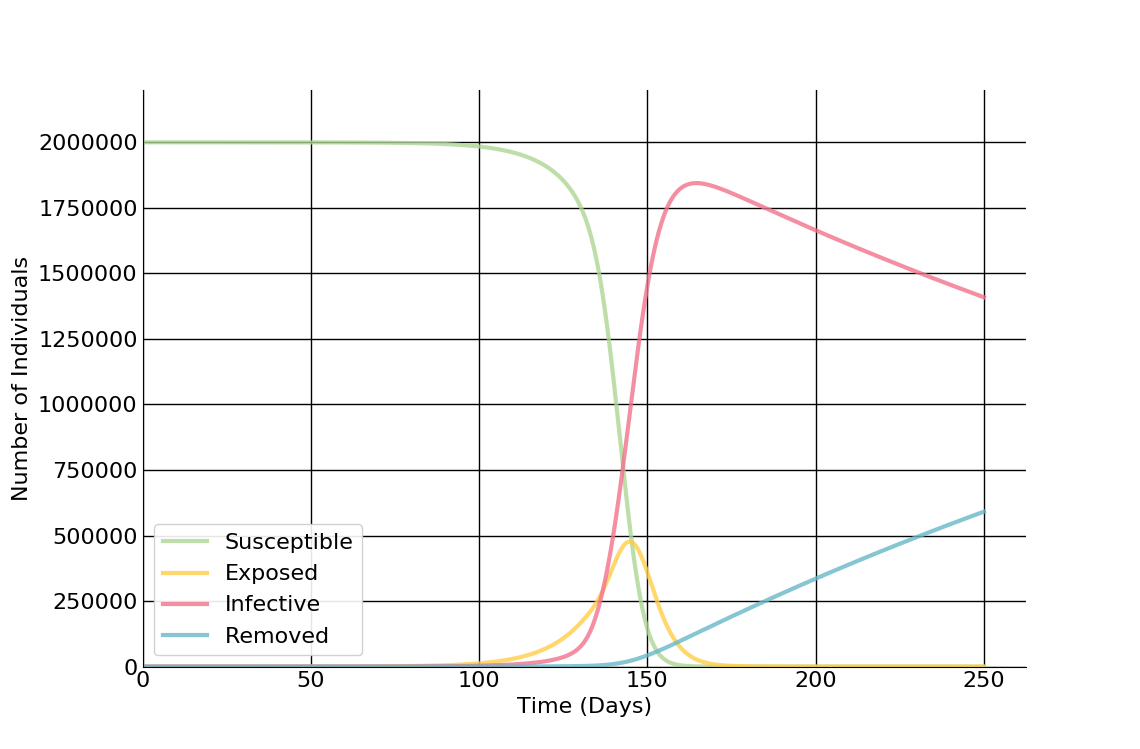
\includegraphics[width=\linewidth]{compartmental-models/rev-trajectory-fill1.png}
	\caption{With default parameters as given in table \ref{tab:parameters-compartments-1}.}
	\label{fig:rev-traj-default}
	\end{subfigure}
	\begin{subfigure}{\textwidth}
	\centering
	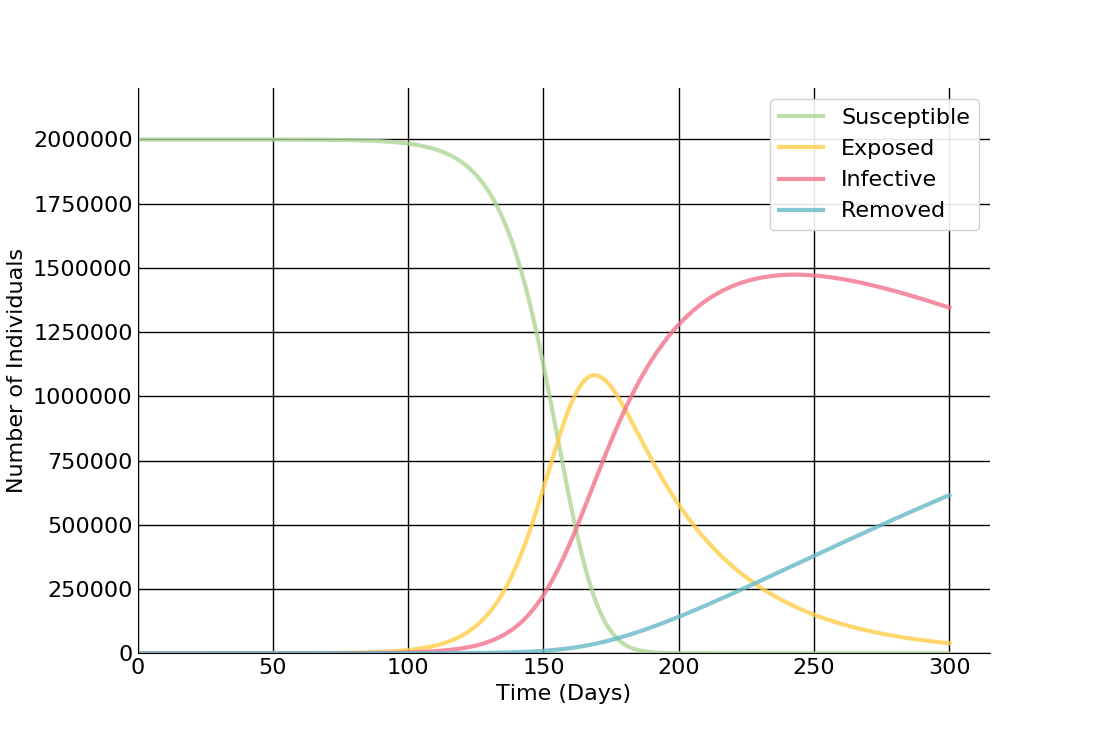
\includegraphics[width=\linewidth]{compartmental-models/rev-trajectory-fill2.png}
	\caption{With default parameters except $\gamma$ altered to $1/500$.
	}
	\label{fig:rev-traj-diff-gamma}
	\end{subfigure}
\caption{Trajectories of the compartmental revolution model.}
\end{figure}
\bigskip
Interestingly this story follows a similar narrative to George Lakey's strategy for nonviolent revolution in `A Manifesto for Nonviolent Revolution'\cite{lakey_1972}. In this he identifies five distinct stages for a successful revolution. The first two are cultural preparation or "conscientization" and building organizations. This educational phase roughly aligns with the `groundwork' stage we observe in our model. He sees confrontation and mass non-cooperation as the second two stages. This has a clear parallel with our 'explosion'. Finally the revolutionaries hope to enter the period `change' which Lakey identifies with the process of developing new institutions.\\
\\
%Returning to the discussion on the validity of our constant $\delta$ assumption we can see that in the early stages when it is mainly zealots converting, the total number of individuals who have been exposed by the time the zealots are the main contributors is very small. In later stages the effect of zealots is overran by the effect of zealots. So the assumption causes only a negligble change.\\
%\\
The simulation confirms the theoretical findings that $R_0$ plays a key role in the existence of an `epidemic'. That is, an increase in the number of active individuals. We can see that for $R_0<1$ no epidemic occurs whilst for values of $R_0$ even slightly above $R_0$ there is an increase in the infective population.
\subsubsection{The role of the contact rate $\beta$}
Further, the importance of $\beta$ is not surprising. A catchy idea catches on. It determines the size of the revolution and also how soon it happens. However, notice the danger of the \textit{good enough} idea as in Fig. \ref{fig:rev-R0-2}. This has $R_0>1$ but only just. As a result, the number of active revolutionaries sustains itself and can even have a small increase. However the amount leaving the cause or being picked off by the regime is almost equal to the amount joining at every point. This is a movement without momentum. It causes no major change but puts people at risk of the regime's wrath. In terms of wasted time and, depending on the nature of individual's removal, lives it is potentially worse than no agitation at all.
%\\
\begin{figure}[h!]
	\centering
	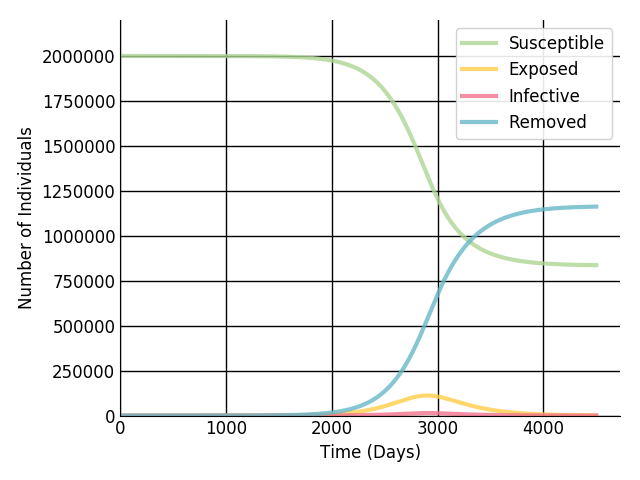
\includegraphics[width=1\linewidth]{compartmental-models/rev-R0-2.png}
	\caption{A graph showing the danger of the `good enough' idea on the revolution model. This has $R_0>1$ but only just.}
	\label{fig:rev-R0-2}
\end{figure}
	
\begin{tcolorbox}
	\paragraph{Lesson for revolutionaries:} Beware of the \textit{good enough} idea. It will not have the momentum needed to cause change. In the meantime it will put you in danger.
%	 If you're going to be active, make sure it's with a catchy idea. Otherwise you might die without seeing anything come of it.
\end{tcolorbox}
\subsubsection{The role of the removal rate $\alpha$}
There is an interesting link between $\alpha$ and $I_{\max}$, the key value we are interested in. Plotting $1/\alpha$ against $I_{\max}$ reveals that $1/\alpha$ has a non-linear effect on the maximum level of infection (Fig. \ref{fig:rev-alpha-not-log}). This suggests a logarithmic relationship. Indeed plotting this confirms this relationship for a large range of parameter values that includes our default value (Fig. \ref{fig:rev-alpha-log}).
\begin{figure}[h!]
	\begin{subfigure}{\textwidth}
		\centering
		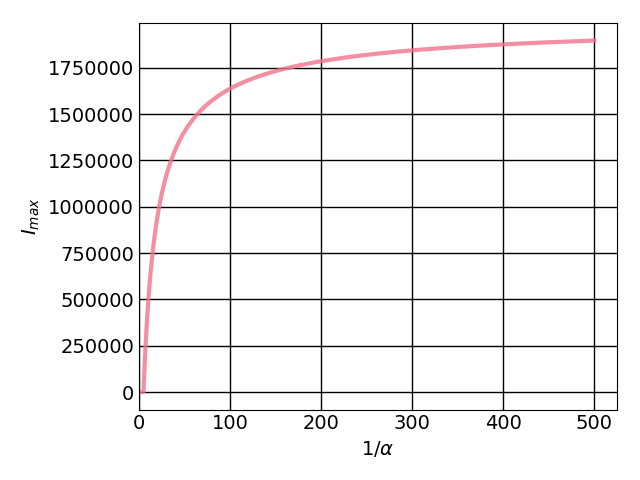
\includegraphics[width=0.8\linewidth]{compartmental-models/rev-alpha-not-log.png}
		\caption{There is a rapid increase in the value of $I_{\max}$ for small increases in $1/\alpha$ but this quickly settles.}
		\label{fig:rev-alpha-not-log}
	\end{subfigure}
	\begin{subfigure}{\textwidth}
		\centering
		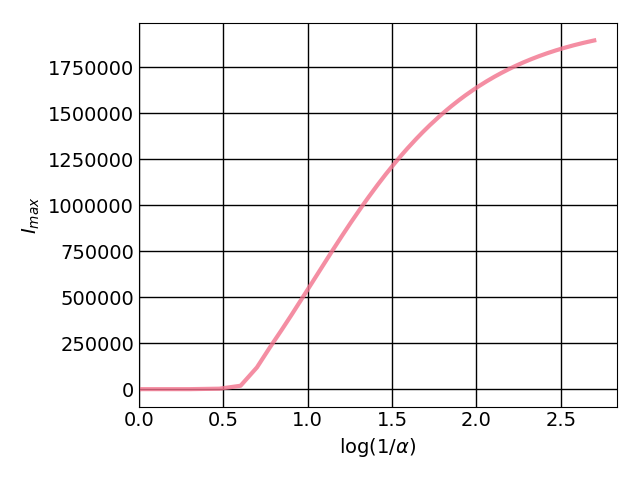
\includegraphics[width=0.8\linewidth]{compartmental-models/rev-alpha-log.png}
		\caption{There is an approximate log relationship between $1/\alpha$ and $I_{\max}$.}
		\label{fig:rev-alpha-log}
	\end{subfigure}
\caption{Graphs showing the effect the value of $1/\alpha$ has on the maximum infected class size. $1/\alpha$ represents the number of days on average it takes for a revolutionary to be removed.}
\end{figure}
%Investigate number of $I_0,E_0$ vs. $\alpha$ removal rate. Might be interesting to see relationship necessary to make something happen.\\
\\
\\
Perhaps even more interesting is the effect of $\alpha$ on the time of the peak of the revolution. Or better said, the lack of effect on it. It might be expected that if more people are leaving the revolution it will take longer to happen. However, this is not the case (Fig. \ref{fig:rev-alpha-time}). If the regime is picking people off any slower than a very fast rate, the peak of the revolution will tend to happen at a similar time. In our model this is around day $162$. In fact, even when $\alpha=0$, that is when no-one leaves the revolution, the peak of the revolution happens on day 162. So as $\alpha\rightarrow0$, the time of peak revolutionary activity $t$ tends to a limit and approaches it very quickly. Hence the time of revolution is not sensitive at all to our choice of $\alpha$.
\begin{figure}[h!]
	\centering
	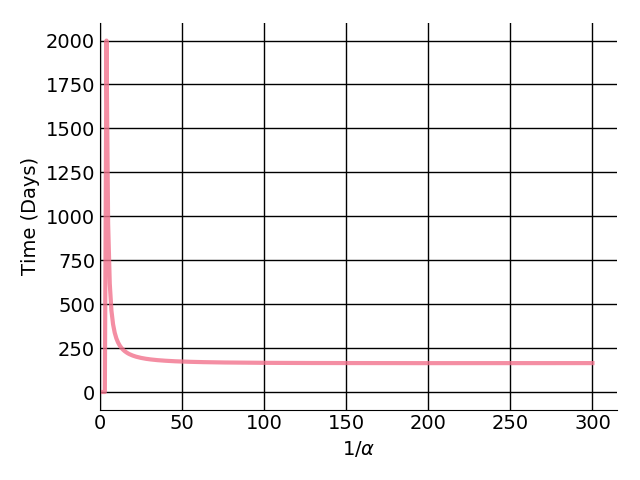
\includegraphics[width=1\linewidth]{compartmental-models/rev-alpha-time.png}
	\caption{A graph showing the lack of effect $\alpha$ has on the time at which the revolution peaks. That is the time $t$ at which $I(t)=I_{\max}$.}
	\label{fig:rev-alpha-time}
\end{figure}
\begin{tcolorbox}
	\paragraph{Lesson for revolutionaries:} The regime can't slow you down (unless they're really, really nasty). However, they will limit the size of the revolution.
\end{tcolorbox}
Note being nasty can be the same as increasing $\alpha$ but this might be intrinsic to the message of the revolutionaries. Therefore it might also involve increasing $\beta$. So tyrants play a tricky balancing act.
\begin{tcolorbox}[colback=removed-colour!30]
	\paragraph{Lesson for tyrants:} Being nasty (i.e. locking people up) will not move the revolution further away. Fortunately for you it will make the revolution smaller. However, it may also make it easier for revolutionaries to gather support against you. Maybe just be nice...?
\end{tcolorbox}
%\paragraph{$\gamma$ and $I_{\max}$}
\subsubsection{The role of the incubation rate $\gamma$}
$\gamma$, the parameter that controls the rate at which non-zealots convert to active revolutionaries, plays a key role in the time it takes for the revolution to happen and, for related reasons, the value of $I_{\max}$. $\gamma$ changes the relative heights of the peaks of $E,I$. If low ($\gamma\sim 1/500$), the growth of $E$ carries on for a long time and has time to grow very high (Fig. \ref{fig:rev-traj-diff-gamma}). Then $\sim1/\gamma$ days later we have the peak of the revolution where $I$ reaches $I_{\max}$. However, as $500$ days is a long time, the build-up to $I_{\max}$ takes a long time. As a result $I_{\max}$ is lower because people were picked off over a longer time. Compare this to Fig. \ref{fig:rev-traj-default}. Similarly, if $\gamma$ is even higher than default ($\gamma\sim1$), $I$ reaches the threshold quickly and then there is no time to remove people during the explosion period and so $I_{\max}\approx N$.
\begin{tcolorbox}
	\paragraph{Lesson for revolutionaries:} Pay attention to the political situation and other peoples' activity. Be ready to join quickly if the time is right.
\end{tcolorbox}
\subsubsection{Shortcomings of the model}
Exploring the simulation also shows the shortcomings of the model. With some parameter values we can witness values of $I<1$ that nevertheless result in an `epidemic'. In a discrete model, less than one revolutionary is no revolutionary. However, the continuity of the compartmental model can allow strange artefacts in which this fraction of a revolutionary manages to cause a revolution. We need something a bit more realistic.